\section{UR and LBR iiwa 7 R800} \label{ch:UR}
\subsubsection{UR5 specifications}
In this section the project takes focus in the differences of the specifications in these 2 cobots. Is one more suitable for the work-cell than the other?

\subsection{UR}

Universal Robots was founded in 2005 by a group of Danish engineers. Their thought was, that every industrial robot on the market was designed to be big, heavy and expensive. Therefore the group decided to make a smaller and more agile kind of industrial robot.\cite{Urhist}\\


The UR is now being used to several different repetitive tasks by big and small companies.
Because UR robots are much smaller and do not have the same force as their bigger counterparts, they can be used in cooperation with humans, which is one of the biggest advantages. This allows the robots to be much more flexible and manageable.\\



These robots can work with humans, and are called collaborative robots/Cobots.\\
Here are the specification for the UR5:\\ 

\begin{figure}[h]
    \centering
    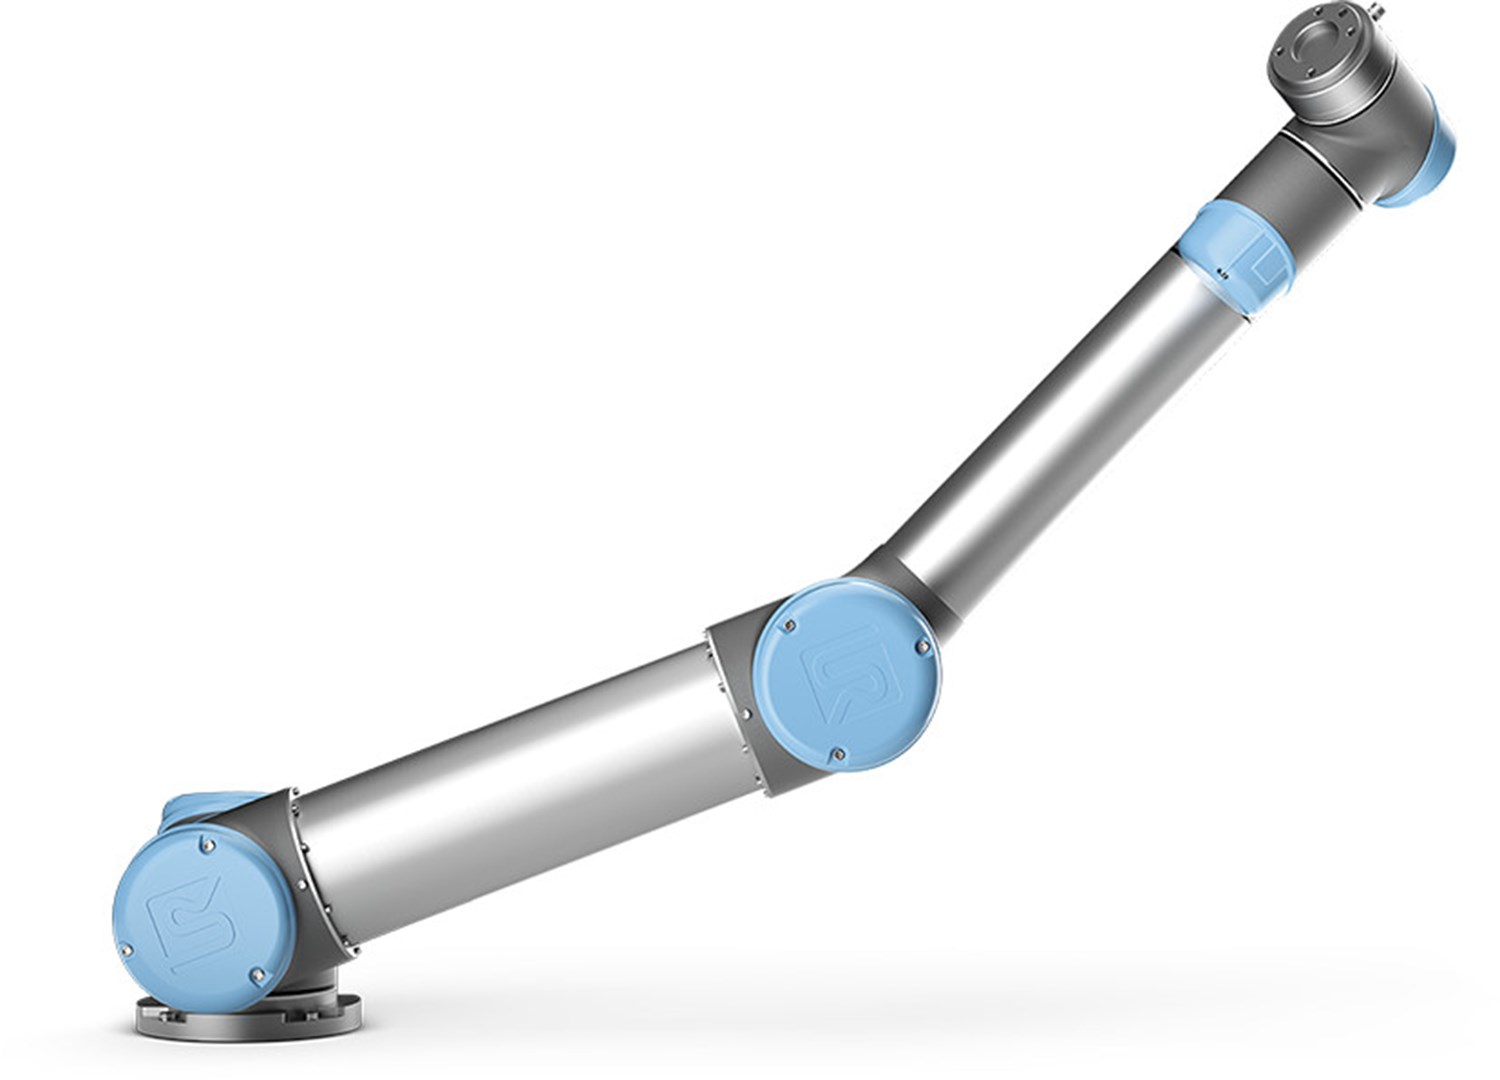
\includegraphics[width=9cm]{UR/UR5pic.jpg}
    \caption{UR5}
    \label{fig:UR5}
\end{figure}

\begin{itemize}
    \item Weight: 18.4 kg.
    \item Payload: 5 kg.
    \item Footprint: 149 mm.
    \item Joints: +/-360 degrees on all the joints.
    \item Operating life: 35,000 Hours.
    \item Speed: joints = 180 degrees/sec, tool = 1 m/sec.
    \item Reach: 850 mm.
    \item Repeatability: +/- 0.1 mm.
\end{itemize}
The materials used on all the cobots are aluminum and plastic\cite{Ur5_about}\cite{UR5_tech}.


\subsubsection{KUKA}

The KUKA company started more than a hundred years ago. They were the first to invent point welding gripper in Germany.\\
As the years goes by the KUKA company writes history by inventing the world first industrial lightweight robot with sensors in every axis.\\

LBR, IIWA and UR are competitors since they have the same market, hence is why this project will take both in to consideration of a possible optimization of the work-cell\cite{KukaHist}.\\


\subsubsection{LBR IIWA 7 R800}
\begin{figure}[h]
    \centering
    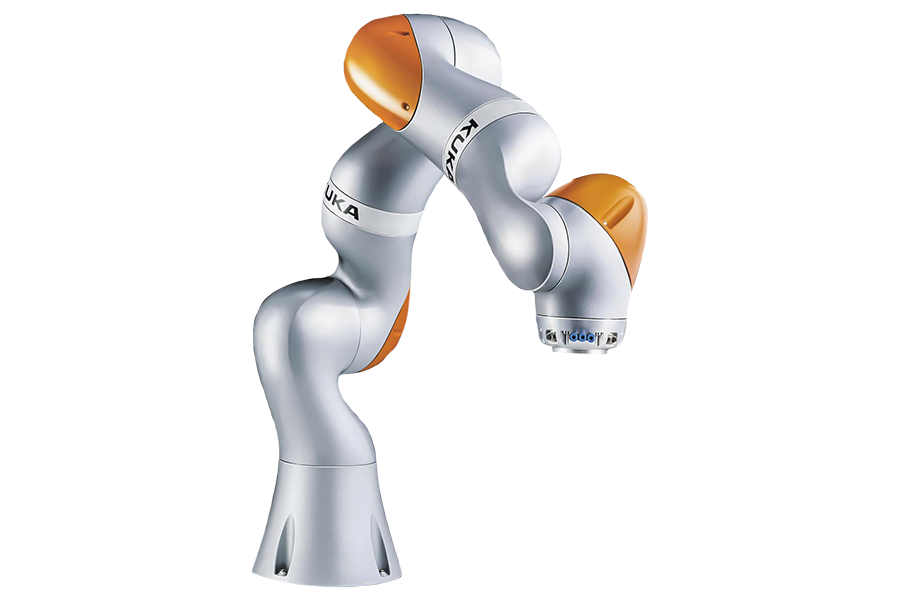
\includegraphics[width=9cm]{UR/1502895088_1.png}
    \caption{LBR IIWA 7 R800}
    \label{fig:LBR IIWA}
\end{figure}

Here are the specification for the LBR iiwa 7 R800:\\

\begin{itemize}
    \item Weight: 23.9 kg.
    \item Payload: 7 kg.
    \item Footprint: 136 mm.
    \item Joints: Ranging from +/-120 degrees to +/-170.
    \item Operating life: 30,000 Hours.
    \item Speed: Joints = 180 degrees/sec
    \item Reach: 800-820 mm
    \item Repeatability: +/- 0.1 mm.
\end{itemize}
\cite{KukaSpec1},\cite{KukaSpec2}.

\subsection{Which cobot is more suitable?}

Given the case-description \ref{ch:case description}, the cobot needs to complete the cyclus of the work-cell within 26 seconds.\\
When inspecting the requirements, a cobot which can do it faster is appropriate for the solution of the project.\\
The speed of the cobots is the same, but UR5 is describing that the end-effector speed is 1m/sec. Which is absolutely vital in a 26 second process.\\
Looking at the joint rotations, the UR5 has the most freedom, while the LBR is invented to rotate with restrictions of maximum +/- 170 degrees.\\
The reach is also important so we can reach every machine in the work-cell.\\

\subsection{Conclusion}

Taking all of the above in to consideration several data can be included in the ideal robot for this case.\\
Having an overview of the different tasks that has to be preformed and using the tools that are given the project can get closer to a conclusion for the robot.\\
The project has focused on two different cobots, 1 from KUKA, and 1 from UR. They are then set up to conclude which has the better specifications. By looking at nothing else than the specifications the most suitable for this case is the UR5.\\

\newpage

